\documentclass{../ucll-slides}
\usepackage{fourier}
\usepackage{bbding}

\usetikzlibrary{shadows,shapes.multipart}

\title{Programming Languages}



\begin{document}

\begin{frame}
  \titlepage
\end{frame}

\begin{frame}
  \frametitle{Programming Languages}
  \begin{center}
    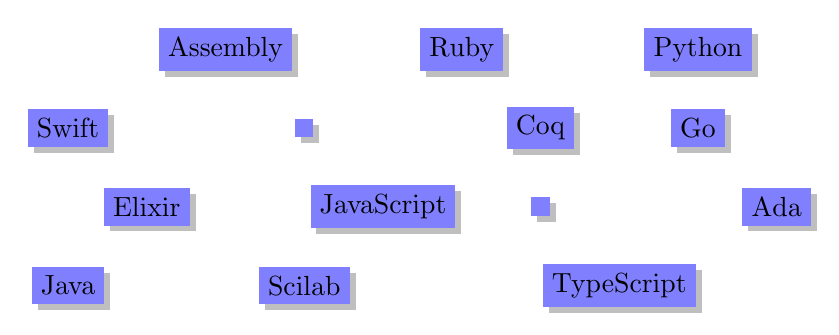
\begin{tikzpicture}[language/.style={fill=blue!50,drop shadow}]
      \node[language] at (0,0) { Java };
      \node[language] at (4,1) { JavaScript };
      \node[language] at (2,3) { Assembly };
      \node[language] at (3,2) { \cpp };
      \node[language] at (6,1) { \csharp };
      \node[language] at (8,3) { Python };
      \node[language] at (5,3) { Ruby };
      \node[language] at (6,2) { Coq };
      \node[language] at (7,0) { TypeScript };
      \node[language] at (9,1) { Ada };
      \node[language] at (3,0) { Scilab };
      \node[language] at (1,1) { Elixir };
      \node[language] at (0,2) { Swift };
      \node[language] at (8,2) { Go };
    \end{tikzpicture}
  \end{center}
  \vskip5mm
  \begin{center}
    Why so many languages?
  \end{center}
\end{frame}



\end{document}
